%% TITLE	Physiological Fluid Mechanics, Summary 2

%% AUTHOR	BINGHUAN W LI (Dept. Chemical Eng/Bio Eng, Imperial)
%%          PETER Y XIE (Dept. Mech Eng, Stanford)

%% compiled in XeLaTeX with Tex Live version 2023.

%% This work is licensed under a Creative Commons Attribution-NonCommercial 4.0 International License.

%=====================================================
% Aug 30, 2024    
% 1. rephrased conservation principles sections, removed
% heat/mass transport eqns, replaced with the table
% 2. add coord. illustrations to NS eqns in sec.2
% 3. sec. 2.1 replaced with a table
%=====================================================

\documentclass[a4paper]{article}
\def\NotesType{1}
\def\summaryNo{2}
\def\finalise{1}
%% TITLE	Physiological Fluid Mechanics, configuration

%% DATE		- Nov 19, 2023     create

%% AUTHOR	BINGHUAN W LI (Dept. Chemical Eng/Bio Eng, Imperial)
%%          PETER Y XIE (Dept. Mech Eng, Stanford)

%% compiled in XeLaTeX with Tex Live version 2023.

%% This work is licensed under a Creative Commons Attribution-NonCommercial 4.0 International License.

\usepackage[sfdefault]{arimo}
\usepackage[left=1.5cm, right=1.5cm, top=2cm, bottom=1.5cm]{geometry}
\usepackage{amsmath, amsfonts, amssymb, cancel}
\usepackage{unicode-math}
\setmathfont
    [    Extension = .otf,
         BoldFont = XITSMath-Bold,
    ]{XITSMath-Regular}

% % \DeclareMathSizes{10}{12}{10}{9}

% \usepackage{siunitx}
\usepackage{enumitem}
\usepackage{xcolor}
    \definecolor{linkcolour}{rgb}{0,0.2,0.6}
\usepackage{hyperref}
\hypersetup{
    colorlinks,
    breaklinks,
    urlcolor=linkcolour,
    linkcolor=linkcolour,
    citecolor=black,
    pdfauthor={Li, Binghuan W},
    }
\usepackage{graphicx, float}
\usepackage{framed}
\usepackage[export]{adjustbox}

\usepackage{fancyhdr}
    \pagestyle{fancy}
    \fancyhf{}
    \lhead{\textsc{Physiological Fluid Mechanics Summary \summaryNo}}
    \rhead{page \thepage}

\usepackage{tcolorbox}

\usepackage{tikz, circuitikz}

\usepackage{multicol}
    \setlength{\columnseprule}{1pt}

\usepackage{lscape}

\usepackage{booktabs}

\usepackage{pifont}

\setlength\parindent{0pt}

\begin{document}
% \include{PFM_supplement1}
\section{Conservation Principles}
\paragraph{Conservation of Linear Momentum (Navier-Stokes)}
\begin{align*}
    \text{\color{gray}(In vector notation)} \quad \quad &  \frac{\partial \mathbf{u}}{\partial t} + (\mathbf{u} \cdot \nabla) \mathbf{u} =  - \frac{1}{\rho} \nabla p + \nu \nabla^2 \mathbf{u} + \mathbf{f} \\[1em]
    \text{\color{gray}(In tensor notation)} \quad \quad & \underbrace{\frac{\partial u_{i}}{\partial t}}_{\text{\ding{192}}} + \underbrace{u_{j}\frac{\partial u_{i}}{\partial x_{j}}}_{\text{\ding{193}}} = \underbrace{- \frac{1}{\rho} \frac{\partial p}{\partial x_{i}}}_{\text{\ding{194}}} + \underbrace{\nu \frac{\partial ^2 u_{i}}{\partial x_{j}\partial x_{j}}}_{\text{\ding{195}}} + \underbrace{ f_{i}}_{\text{\ding{196}}}
\end{align*}
        
    \begin{center}
    \begin{tabular}{llll}
        \text{\ding{192}} & rate of change of speed (unsteady)&
        \text{\ding{193}} & convective acceleration \\
        \text{\ding{194}} & pressure gradient  &
        \text{\ding{195}} & diffusion (viscous) acceleration \\
        \text{\ding{196}} & body force: gravitational, EM, \textit{etc.}\\
    \end{tabular}
    \end{center}

    \underline{Comments}:
    \begin{itemize}
        \item[-] Term \text{\ding{192}} and \text{\ding{193}} together represent the \textbf{material derivative} of $\mathbf{u}$, which is the total acceleration of a fluid element.

        \item[-] Term \text{\ding{194}} and \text{\ding{195}}  represent the internal forces acting on a fluid element. Term \text{\ding{196}} is the body (external) force acting on a fluid element.
        
        \item[-] The N-S is non-linear due to the presence of term \text{\ding{193}}; hence, N-S cannot be decomposed using basis functions (\textit{e.g.} Fourier series). 

        \item[-] There are many possible formulations of the N-S equation. The abovementioned formulation assumes the fluid is incompressible (constant $\rho$) and Newtonian (constant $\mu$, hence $\nu=\mu/\rho$ is also constant).
    \end{itemize}

\paragraph{Other Transport Phenomena} Transport of heat, mass, and momentum share similar mathematical frameworks.

\begin{table}[H]
    \centering
    \begin{tabular}{cccc}
    \toprule
        \textbf{Transport of ...} & \textbf{Governing Equation} & \textbf{``Diffusivity''} & \textbf{``Source''} \\
    \midrule
        Heat & $\displaystyle \frac{\partial T}{\partial t} + (\mathbf{u} \cdot \nabla) T = \alpha \nabla^2 T + \dot{S}_T$ & $\displaystyle \alpha = k/\rho c_p$ & $\dot{S}_{T} = \dot{S}_{v}/\rho c_p$ \\ [.5cm]
        
        Mass & $\displaystyle \frac{\partial C}{\partial t} + (\mathbf{u} \cdot \nabla) C = \mathcal{D} \nabla^2 C + \dot{S}_C$ & $\mathcal{D}$ & $\dot{S}_{C}$ \\ [.5cm]
        
        Momentum (N-S) & $\displaystyle \frac{\partial \mathbf{u}}{\partial t} + (\mathbf{u} \cdot \nabla) \mathbf{u} = \nu \nabla^2 \mathbf{u} + \dot{S}_v$ & $\displaystyle \nu = \mu/\rho$ & $\dot{S}_{v} = (-\nabla p + \rho \mathbf{f})/\rho$ \\
    \bottomrule
    \end{tabular}
\end{table}

\section{The Continuity and Navier-Stokes Equations}
\paragraph{Cartesian Coordinates} $\mathbf{u} \in [u, v, w]$ \\

\begin{minipage}{.75\textwidth}
\begin{itemize}
    \item Continuity Equation:
    \[\frac{\partial u}{\partial x} + \frac{\partial v}{\partial y} + \frac{\partial w}{\partial z}=0\]
    
    \item Momentum Equations:
    \begin{align*}
        \boldsymbol{x:} \quad & \rho \bigg(\frac{\partial u}{\partial t} + u \frac{\partial u}{\partial x} + v\frac{\partial u}{\partial y} + w\frac{\partial u}{\partial z} \bigg) = -\frac{\partial p}{\partial x} + \mu \bigg(\frac{\partial^{2} u}{\partial x^{2}} + \frac{\partial^{2} u}{\partial y^{2}} + \frac{\partial^{2} u}{\partial z^{2}}\bigg) + \rho f_{x} \\[1em]
        \boldsymbol{y:} \quad & \rho \bigg(\frac{\partial v}{\partial t} + u \frac{\partial v}{\partial x} + v\frac{\partial v}{\partial y} + w\frac{\partial v}{\partial z} \bigg) = -\frac{\partial p}{\partial y} + \mu \bigg(\frac{\partial^{2} v}{\partial x^{2}} + \frac{\partial^{2} v}{\partial y^{2}} + \frac{\partial^{2} v}{\partial z^{2}}\bigg) + \rho f_{y} \\[1em]
        \boldsymbol{z:} \quad & \rho \bigg(\frac{\partial w}{\partial t} + u \frac{\partial w}{\partial x} + v\frac{\partial w}{\partial y} + w\frac{\partial w}{\partial z} \bigg) = -\frac{\partial p}{\partial z} + \mu \bigg(\frac{\partial^{2} w}{\partial x^{2}} + \frac{\partial^{2} w}{\partial y^{2}} + \frac{\partial^{2} w}{\partial z^{2}}\bigg) + \rho f_{z}
    \end{align*}
\end{itemize}
\end{minipage}
\begin{minipage}{.25\textwidth}
    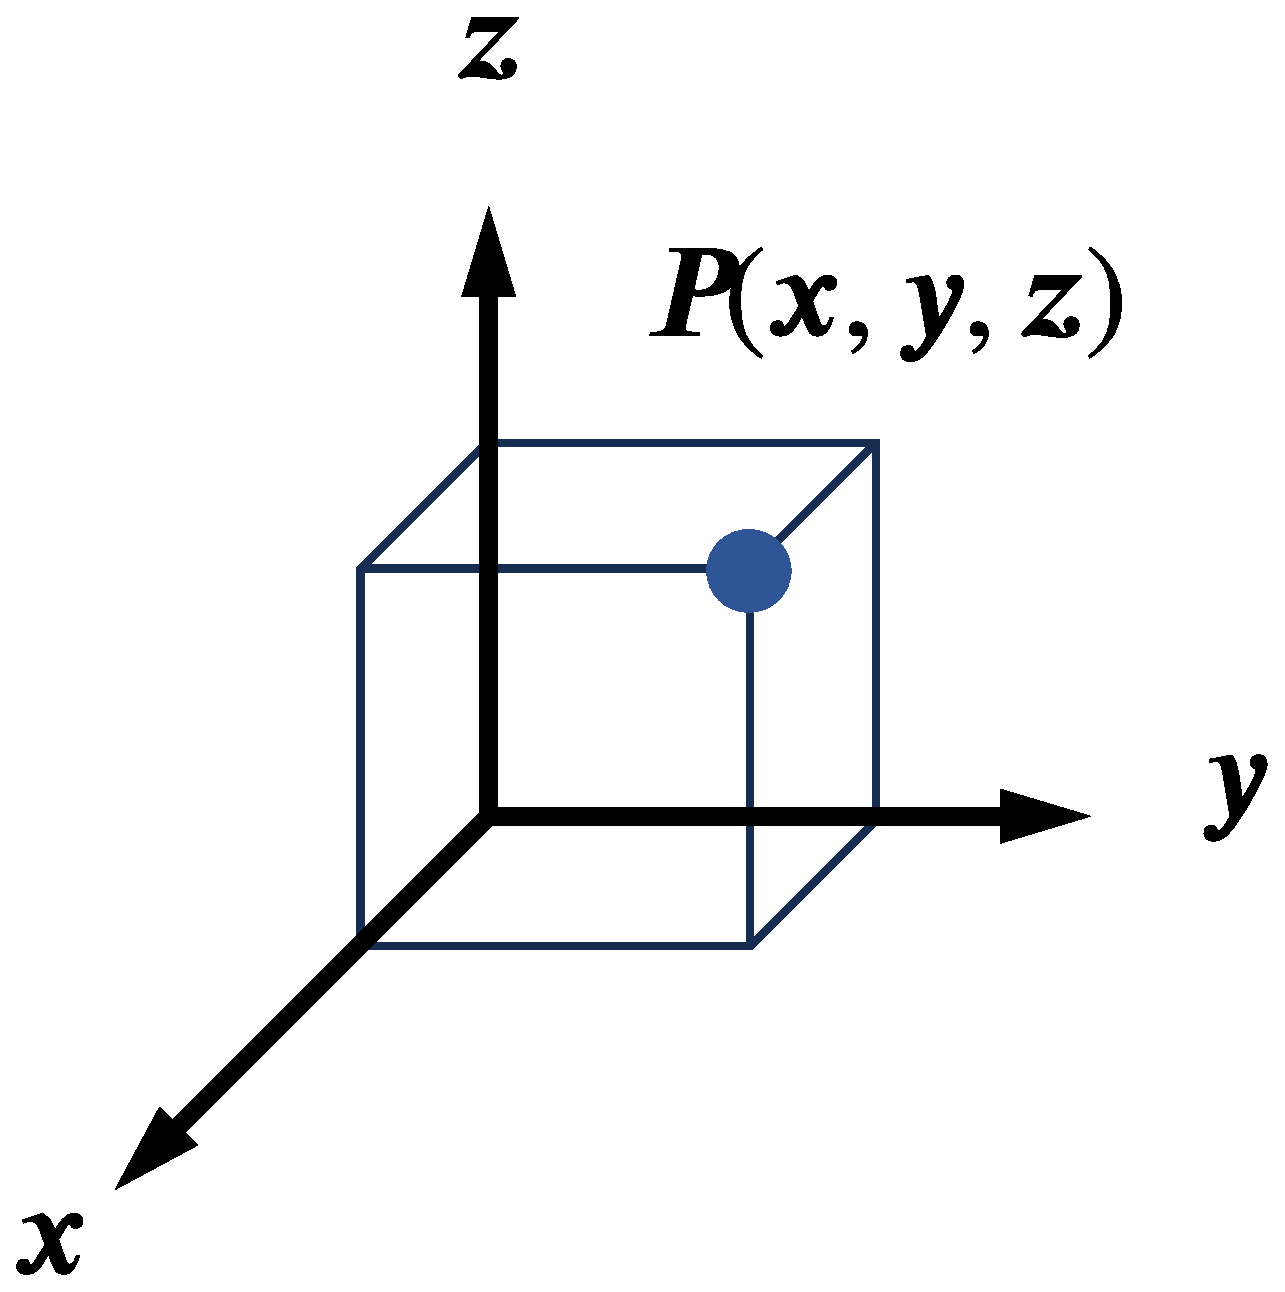
\includegraphics[width=.9\textwidth]{img/cartesian_coord_sys.eps}
\end{minipage}


\paragraph{Cylindrical Coordinates} $\mathbf{u} \in [u_r, u_\theta, u_z]$

\begin{itemize}
    \item Continuity Equation:
    \[\frac{1}{r}\frac{\partial ru_{r}}{\partial r} + \frac{1}{r}\frac{\partial u_{\theta}}{\partial \theta} + \frac{\partial u_{z}}{\partial z}=0\]
\end{itemize}

\begin{minipage}{.75\textwidth}
\begin{itemize}
    \item Momentum Equations:
    
    \begin{equation*}
    \begin{split}
        \boldsymbol{r:} \ & \rho \bigg(\frac{\partial u_{r}}{\partial t} + u_{r} \frac{\partial u_{r}}{\partial r} + \frac{u_{\theta}}{r}\frac{\partial u_{r}}{\partial \theta} + u_{z}\frac{\partial u_{r}}{\partial z} - \frac{u_{\theta}^{2}}{r} \bigg) \\
        & = -\frac{\partial p}{\partial r} + \mu \bigg[ \frac{1}{r}\frac{\partial}{\partial r} \bigg(r \frac{\partial u_{r}}{\partial r}\bigg) + \frac{1}{r^{2}} \frac{\partial^{2} u_{r}}{\partial \theta^{2}} + \frac{\partial^{2} u_{r}}{\partial z^{2}} - \frac{u_{r}}{r^{2}} - \frac{2}{r^{2}}\frac{\partial u_{\theta}}{\partial \theta}\bigg] + \rho f_{r}
    \end{split}
    \end{equation*}
    
    \begin{equation*}
    \begin{split}
        \boldsymbol{\theta:} \ & \rho \bigg(\frac{\partial u_{\theta}}{\partial t} + u_{r} \frac{\partial u_{\theta}}{\partial r} + \frac{u_{\theta}}{r} \frac{\partial u_{\theta}}{\partial \theta} + u_{z}\frac{\partial u_{\theta}}{\partial z} + \frac{u_{r}u_{\theta}}{r} \bigg) \\
        & = -\frac{1}{r} \frac{\partial p}{\partial \theta} + \mu \bigg[ \frac{1}{r}\frac{\partial}{\partial r} \bigg(r \frac{\partial u_{\theta}}{\partial r}\bigg) + \frac{1}{r^{2}} \frac{\partial^{2} u_{\theta}}{\partial \theta^{2}} + \frac{\partial^{2} u_{\theta}}{\partial z^{2}} - \frac{u_{\theta}}{r^{2}} + \frac{2}{r^{2}}\frac{\partial u_{r}}{\partial \theta}\bigg] + \rho f_{\theta}
    \end{split}
    \end{equation*}
    
    \begin{equation*}
    \begin{split}
        \boldsymbol{z:} \ & \rho \bigg(\frac{\partial u_{z}}{\partial t} + u_{r} \frac{\partial u_{z}}{\partial r} + \frac{u_{\theta}}{r}\frac{\partial u_{z}}{\partial \theta} + u_{z}\frac{\partial u_{z}}{\partial z} \bigg) \\
        & = -\frac{\partial p}{\partial z} + \mu \bigg[ \frac{1}{r}\frac{\partial}{\partial r} \bigg(r \frac{\partial u_{z}}{\partial r}\bigg) + \frac{1}{r^{2}} \frac{\partial^{2} u_{z}}{\partial \theta^{2}} + \frac{\partial^{2} u_{z}}{\partial z^{2}} \bigg] + \rho f_{z}
    \end{split}
    \end{equation*}
\end{itemize}
\end{minipage}
\begin{minipage}{.25\textwidth}
    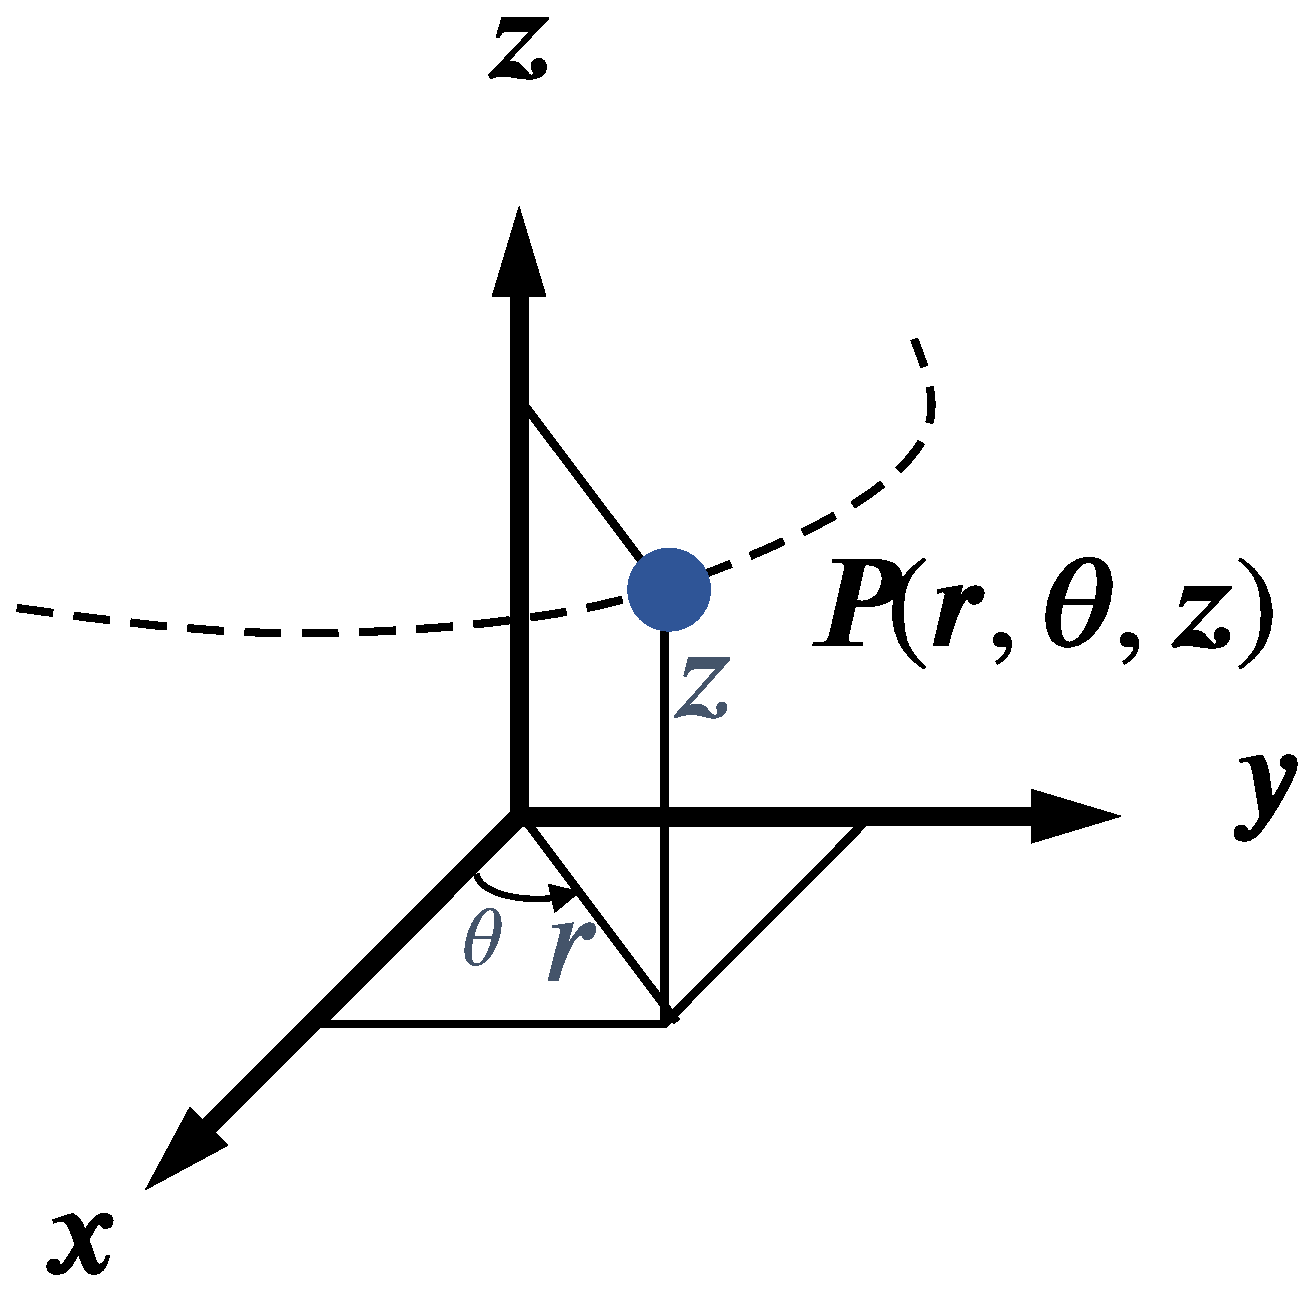
\includegraphics[width=.9\textwidth]{img/cylind_coord_sys.eps}
\end{minipage}

\vspace{.3cm}
% \paragraph{Spherical Coordinates} $\mathbf{u} \in [u_r, u_\theta, u_\phi]$ \\

% \begin{minipage}{.75\textwidth}
% \begin{itemize}
%     \item Continuity Equation:
%     \[\frac{1}{r^{2}}\frac{\partial r^{2}u_{r}}{\partial r} + \frac{1}{r \sin \theta}\frac{\partial u_{\theta}\sin \theta}{\partial \theta} + \frac{1}{r \sin \theta}\frac{\partial u_{\phi}}{\partial \phi}=0\]
    
%     \item Momentum Equations:
%     \begin{equation*}
%     \begin{split}
%     \boldsymbol{r:} \ & \rho \bigg(\frac{\partial u_{r}}{\partial t} + u_{r} \frac{\partial u_{r}}{\partial r} + \frac{u_{\theta}}{r}\frac{\partial u_{r}}{\partial \theta} + \frac{u_{\phi}}{r \sin \theta} \frac{\partial u_{r}}{\partial \phi} - \frac{u_{\theta}^{2}+u_{\phi}^{2}}{r} \bigg)  \\ 
%     & = -\frac{\partial p}{\partial r} + \mu \bigg( \nabla^{2}u_{r} - \frac{2u_{r}}{r^{2}} - \frac{2}{r^{2}\sin \theta}\frac{\partial}{\partial \theta}(u_{\theta}\sin\theta) + \frac{2}{r^{2}\sin\theta}\frac{\partial u_{\phi}}{\partial \phi} \bigg) + \rho f_{r}
%     \end{split}  
%     \end{equation*}
    
%     \begin{equation*}
%     \begin{split}
%     \boldsymbol{\theta:} \ & \rho \bigg(\frac{\partial u_{\theta}}{\partial t} + u_{r} \frac{\partial u_{\theta}}{\partial r} + \frac{u_{\theta}}{r} \frac{\partial u_{\theta}}{\partial \theta} + \frac{u_{\phi}}{r\sin \theta} \frac{\partial u_{\theta}}{\partial \phi} + \frac{u_{r}u_{\theta}-u_{\phi}^{2}\cot\theta}{r} \bigg) \\
%     & = -\frac{1}{r}\frac{\partial p}{\partial \theta} + \mu \bigg( \nabla^{2}u_{\theta} - \frac{u_{\theta}}{r^{2}\sin^{2}\theta} + \frac{2}{r^{2}}\frac{\partial u_{r}}{\partial \theta} - \frac{2\cos \theta}{r^{2}\sin^{2}\theta}\frac{\partial u_{\phi}}{\partial \phi} \bigg) + \rho f_{\theta}
%     \end{split}  
%     \end{equation*}
    
%     \begin{equation*}
%     \begin{split}
%     \boldsymbol{\phi:} \ & \rho \bigg(\frac{\partial u_{\phi}}{\partial t} + u_{r} \frac{\partial u_{\phi}}{\partial r} + \frac{u_{\theta}}{r} \frac{\partial u_{\phi}}{\partial \theta} + \frac{u_{\phi}}{r\sin \theta} \frac{\partial u_{\phi}}{\partial \phi} + \frac{u_{r}u_{\phi}+u_{\phi}u_{\theta}\cot\theta}{r} \bigg) \\
%     & = -\frac{1}{r\sin\theta}\frac{\partial p}{\partial \phi} + \mu \bigg( \nabla^{2}u_{\phi} - \frac{u_{\phi}}{r^{2}\sin^{2}\theta} + \frac{2}{r^{2}\sin \theta}\frac{\partial u_{r}}{\partial \phi} - \frac{2\cos \theta}{r^{2}\sin^{2}\theta}\frac{\partial u_{\theta}}{\partial \phi} \bigg) + \rho f_{\phi}
%     \end{split}  
%     \end{equation*}
% \end{itemize}
% \end{minipage}
% \begin{minipage}{.25\textwidth}
%     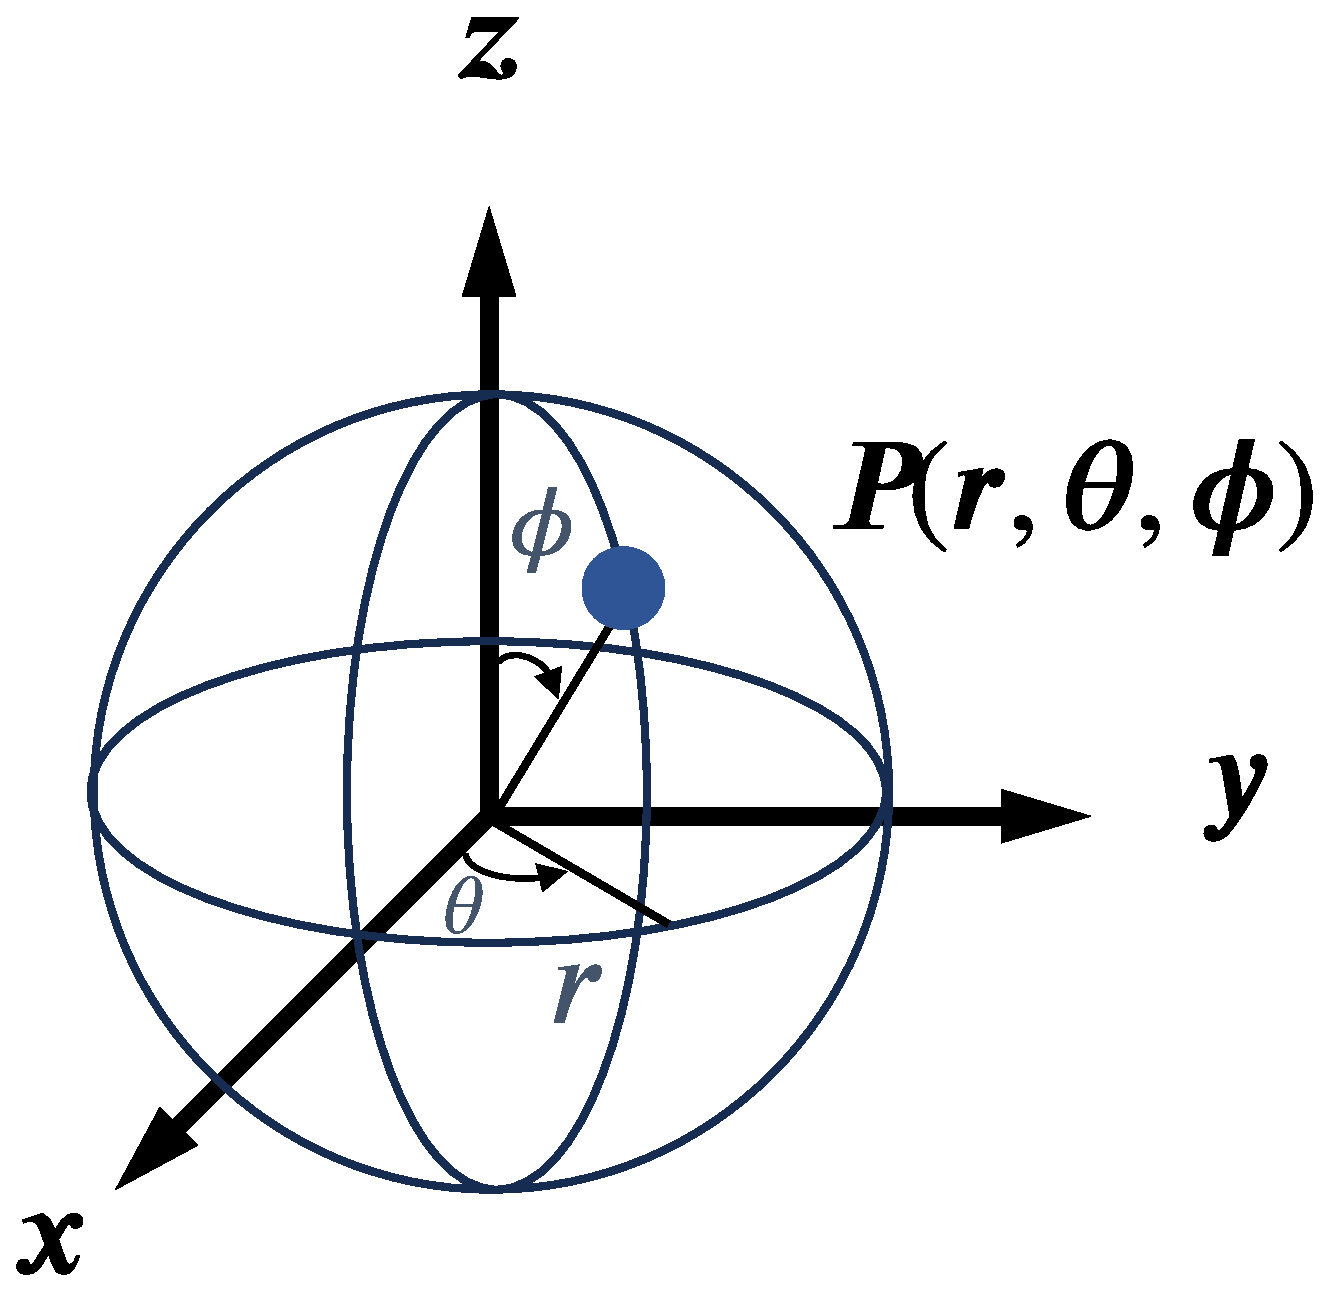
\includegraphics[width=.9\textwidth]{img/sphere_coord_sys.eps}
% \end{minipage}


\subsection{Assumptions to Simplify the Navier-Stokes Equations}

\begin{table}[H]
    \centering
    \begin{tabularx}{\textwidth}{m{.2\textwidth} m{.2\textwidth} m{.15\textwidth} m{.35\textwidth}}
        \toprule
        \textbf{Assumption} & \textbf{Applicable to...} & \textbf{Mathematical expression} & \textbf{Note} \\ 
        \midrule
        Steady & Cartesian, cylindrical, spherical & $\frac{\partial}{\partial t} = 0$ & \\[.5cm]
        Fully developed & Cartesian, cylindrical, spherical & $\frac{\partial \mathbf{u}}{\partial n} = 0$ & "Fully developed" indicates the velocity profile is independent of the location, not pressure. \\[.5cm]
        Axisymmetric & cylindrical, spherical & $\frac{\partial}{\partial \theta} = 0$ & \\[.5cm]
        Spherical symmetric & spherical & $\frac{\partial}{\partial \theta} = 0, \quad \frac{\partial}{\partial \phi} = 0$ & \\[.5cm]
        No swirl & cylindrical, spherical & $u_{\theta} = 0$ & \\[.5cm]
        Two-dimensional (with $z$-direction absent) & Cartesian & $u_z = 0, \quad \frac{\partial}{\partial z} = 0$ & For fluid flow in cylindrical coordinates, axisymmetric assumption simplifies the 3D flow to 2D flow. \\[.5cm]
        Neglect body force & Cartesian, cylindrical, spherical & $\mathbf{f} = 0$ & \\ 
        \bottomrule
    \end{tabularx}
    \label{tab:flow_assumptions}
\end{table}
    
\vfill
{\small \color{gray}Drafted by B. Li, H. El Nashar, and C. H. Yap,  \today}
% \thispagestyle{empty}
\newgeometry{margin=1.8cm}
\mbox{}
\vfill    
\begin{figure}[H]
    \includegraphics[right]{images/by-nc.eps}
\end{figure}
\textit{This work is licensed under a Creative Commons Attribution-NonCommercial 4.0 International License.}


\end{document}